\documentclass{article}

%\usepackage[left=2.5cm,right=2.5cm,top=1.5cm,bottom=1.5cm]{geometry}
\usepackage{anysize}
\usepackage{graphicx}
\usepackage{parskip}
\usepackage{amsmath, amsthm, amssymb, amsfonts}

\usepackage{times}

\usepackage[utf8]{inputenc} % this is needed for umlauts
\usepackage[german]{babel} % this is needed for umlauts
\usepackage[T1]{fontenc}    % this is needed for correct output of umlauts in pdf

\usepackage[font=small,labelfont=bf]{caption}

\newcommand{\piMIN}{\pi_\text{MIN}}
\newcommand{\piMAX}{\pi_\text{MAX}}
\newcommand{\pimin}{\pi_\text{min}}
\newcommand{\pimax}{\pi_\text{max}}
\newcommand{\phiMIN}{\varphi_\text{MIN}}
\newcommand{\phiMAX}{\varphi_\text{MAX}}
\newcommand{\phimin}{\varphi_\text{min}}
\newcommand{\phimax}{\varphi_\text{max}}
\newcommand{\LMAX}{L_\text{MAX}}
\newcommand{\LMIN}{L_\text{MIN}}
\newcommand{\Lmax}{L_\text{max}}
\newcommand{\pin}{p_\text{in}}

\begin{document}

\section*{Verdichtermodellierung}

Verdichter sind von allen modellierten Elementen die kompliziertesten. Über das sogenannte Kennfeld wird im Fluss-Druckverhältnis-Diagramm derjenige Bereich definiert, der für den jeweiligen Verdichter erlaubt ist solange er aktiv ist, solange er also Gas verdichtet.

Dabei ist zu beachten, das der Begriff Kennfeld hier etwas anders benutzt wird als allgemein üblich. Normalerweise begreift man einen Verdichter als eine Maschineneinheit aus Antrieb und dem eigentlichen Erdgasverdichter. Jeder der beiden Teile hat dabei sein eigenes Kennfeld. In unserem Modell vereinfachen wir die Sache sehr: Die maximale und minimale Leistung des Antriebs werden zusammen mit dem Kennfeld des Verdichters in ein gemeinsames Diagramm aufgenommen.

\section{Aufbau des Kennfelds}
Unser Kennfeld (siehe Abb. \ref{fig:kf}) ist ein x-y-Diagramm, das den erlaubten Bereich des Verdichterzustands definiert. Auf der x-Achse steht der Betriebsvolumenfluss $\varphi$ durch den Verdichter, auf der y-Achse das Druckverhältnis $\pi:=\frac{p_{\text{out}}}{p_{\text{in}}}$ aus Ausgangs- und Eingangsdruck.

%\begin{equation}
%\pi:=\frac{p_{\text{out}}}{p_{\text{in}}}
%\label{eq:pi}
%\end{equation}


\begin{figure}[!ht]
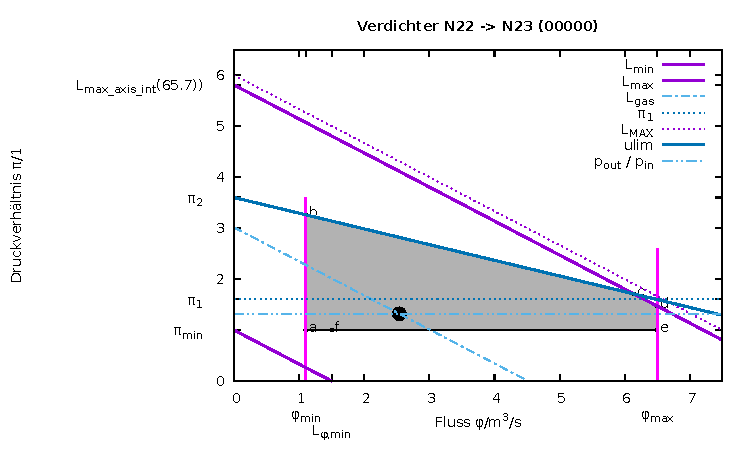
\includegraphics[width=0.9\textwidth]{Example_Compressor_Wheel_Map.pdf}
\caption{Für unsere Zwecke vereinfachtes Verdichterkennfeld, das neben den Kenndaten für den eigentlichen Verdichter auch die Antriebsleistung enthält.}
\label{fig:kf}
\end{figure}

Im weiteren Verlauf dieses Artikels wird die Bezeichnung {\em Kennfeld} mal für das x-y-Diagramm und mal für den in diesem Diagramm erlaubten Bereich des Verdichterzustands verwendet. Aus dem Kontext sollte aber ersichtlich sein, wie die Bezeichnung jeweils verwendet wird.

Auf der x-Achse sind zwei Konstanten definiert, die das Kennfeld links und rechts begrenzen, 
$\varphi_\text{min}$ ist der minimal zulässige Fluss und $\phimax$ der maximal zulässige. Auf der y-Achse definiert $\pimin$ das minimal zulässige Druckverhältnis, es hat üblicherweise den Wert 1.

\section{Antriebsleistungen}

Für einen Verdichter sind drei Leistungen definiert, die durch parallele Geraden modelliert werden:

\begin{enumerate}

\item Minimalleistung; Gerade durch $(0,\piMIN)$ und $(\phiMIN,0)$
$$L_\text{MIN}: \begin{pmatrix} 0 \\ \piMIN \end{pmatrix} + \lambda \begin{pmatrix} \phiMIN - 0 \\ 0 - \piMIN \end{pmatrix},\text{ bzw. } \LMIN(\varphi)=-\frac{\piMIN}{\phiMIN}\varphi+\piMIN$$

\item Absolute Maximalleistung; Parallele zu $L_\text{MIN}$ durch $(0,\pi_{\text{MAX}})$
$$L_\text{MAX}: \begin{pmatrix} 0 \\ \pi_{\text{MAX}} \end{pmatrix} + \lambda \begin{pmatrix} \phiMIN - 0 \\ 0 - \piMIN \end{pmatrix},\text{ bzw. } L_{\text{MAX}}(\varphi)=-\frac{\piMIN}{\phiMIN}\varphi+\piMAX$$

\item Aktuelle Maximalleistung; Parallele zu $L_\text{MIN}$ durch $(0,\pimax)$
$$\Lmax(\pimax): \begin{pmatrix} 0 \\ \pimax \end{pmatrix} + \lambda \begin{pmatrix} \phiMIN - 0 \\ 0 - \piMIN \end{pmatrix},\text{ bzw. } L_{\text{max}}(\varphi)=-\frac{\piMIN}{\phiMIN}\varphi+\pimax$$

\end{enumerate}

Die aktuelle Maximalleistung hängt von einer Funktion $\pimax$ vom aktuellen Eingangsdruck $p^\text{in}$ ab.
$$\pimax: p_\text{in} \longmapsto \piMAX \left( (\eta - 1) \frac{\pin - \pin^{\text{min}}}{\pin^{\text{max}} - \pin^{\text{min}}} + 1 \right)$$
Der Wirkungsgrad $\eta$ wird dazu genutzt die Abhängigkeit der aktuellen Maximalleistung vom Eingangsdruck zu modellieren.
 
\section{Kennfeldgrenzen}

Die Gerade U durch die Punkte $(0, \pi_2)$ und $(\phimax, \pi_1)$ dient dazu, das Kennfeld nach oben zu begrenzen.
Dabei beschreibt $\pi_2$  gewissermaßen das maximale Druckverhältnis bei Nullfluss und $\pi_1$ das minimale Druckverhältnis bei maximalem Fluss.
$$U: \begin{pmatrix} 0 \\ \pi_2 \end{pmatrix} + \lambda \begin{pmatrix} \phimax - 0 \\ \pi_1 - \pi_2 \end{pmatrix},\text{ bzw. } U(\varphi)=\frac{(\pi_1-\pi_2)}{\phimax}\varphi+\pi_2$$


Das Kennfeld ist ein Sechseck mit den Eckpunkten a bis f, die folgendermaßen definiert sind:
\begin{description}

\item[a]  Punkt $(\varphi_\text{min},L_\text{MIN}(\varphi_\text{min}))$
\item[b]  Punkt $(\varphi_\text{min}, U(\phimin))$
\item [c] Schnittpunkt der beiden Geraden $U$ und $\Lmax$
\item [d] Punkt $(\phimax, \Lmax(\phimax))$
\item [e] Punkt ($\phimax, \pimin)$  
\item [f] Punkt $(\LMIN^{-1}(\pimin), \pimin)$ 

\end{description}


\section{ Bestimmung des Arbeitspunktes}

Der Dispatcher-Agent darf sich wünschen, ob der Verdichter aktiv ist
oder nicht. Dem Wunsch auf Inaktivität wird immer entsprochen, dem auf
Aktivität nicht.

Der Arbeitspunkt $A$ eines aktiven Verdichters muss immer im Kennfeld $K$
liegen und immer auf $\pi$. Falls diese beiden Mengen disjunkt sind, wenn $\pi$ also nicht in $K$ liegt, so ist der Verdichter zwingend inaktiv.

Der Wunsch auf Aktivität muss immer mit einer Wunschleistung $W$ verbunden
sein. $W$ liegt zwischen 0\% und 100\% und wird vom Simulator auf eine
Leistung $L$ umgerechnet, die zwischen $L_\text{MIN}$ und $\Lmax$ liegt.

Es gibt immer einen Schnittpunkt $S$ von $L$ und $\pi$. Liegt $S$ in $K$, so ist $A = S$. Liegt $S$ nicht in $K$, so ist $S$ der nächstgelegene Randpunkt von $K$, der auf
$\pi$ liegt. Per Konstruktion muss es einen solchen Punkt geben:

\begin{itemize}
\item Bilde $D$ als Schnittstrecke von $\pi$ und $K$.
\item Bilde $S$ als Schnittpunkt von $\pi$ und $L$.
\item Dann ist $A$ der $S$ nächstgelegene Punkt aus $D$.
\end{itemize}

\end{document}
